\subsection{LQG mit Folgeregelung}
    Analog zum LQR-Regler können wir den Gleichgewichtspunkt nach $\{x_\infty,\, u_\infty\}$ verschieben.
    
    Das resultierende Stellsignal ist
    \begin{equation*}
        u(t) = u_\infty - K\cdot(\widehat{x}(t)-\widehat{x}_\infty) = u_\infty - K\cdot(\widehat{x}(t)-x_\infty)
    \end{equation*}
    Da der Fehler $e(t)= x(t)-\widehat{x}(t)$ asymptotisch zu null konvergiert gilt $x_\infty = \widehat{x}_\infty$.
    
    \begin{figure}[H]
        \centering
        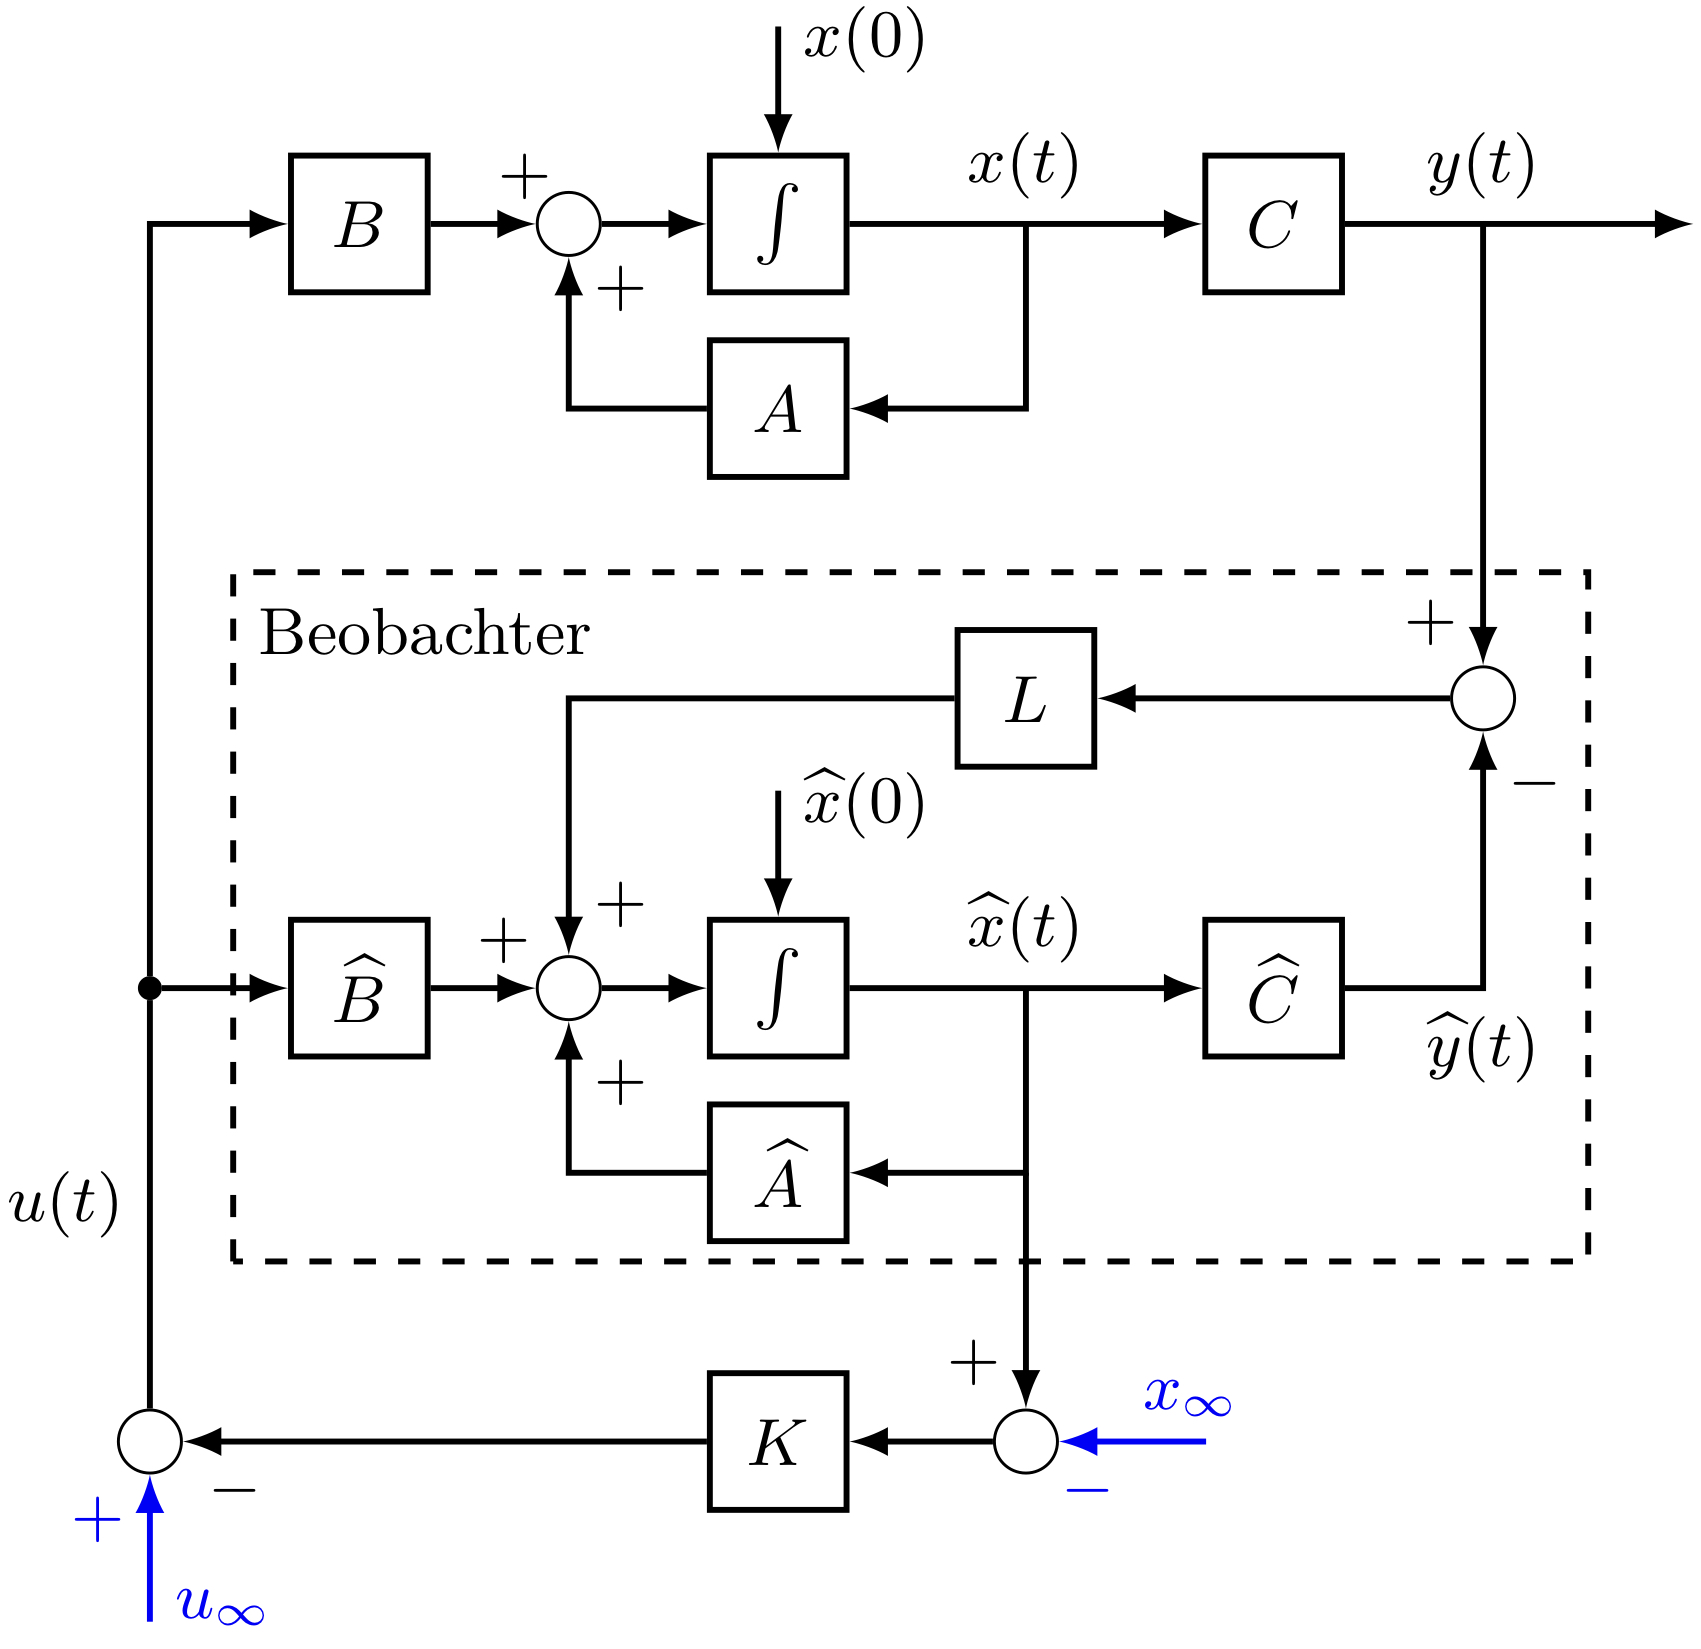
\includegraphics[width = 0.6\linewidth]{images/10/LQG_Folg.jpeg}
        \caption{LQG mit Folgeregelung durch $\{x_\infty,\, u_\infty\}$}
        \label{fig:lqgfolgeregelung}
    \end{figure}
    
    \subsubsection{Folgeregelung durch Vorsteuerung} \label{s:LQGIFolgeregelung}
        Die Struktur aus Abb. \ref{fig:lqgfolgeregelung} kann auch durch eine Folgeregelung auf die Referenz $r(t)$ umsetzen. 
        
        \begin{equation*}
            r(t) = \begin{bmatrix}r_1\\r_2\\\hdots\\r_m\end{bmatrix},\quad
            r(t) = \underbrace{y_\infty}_{= \textnormal{Const.}} = C\cdot x_\infty
        \end{equation*}
        \begin{figure}[H]
            \centering
            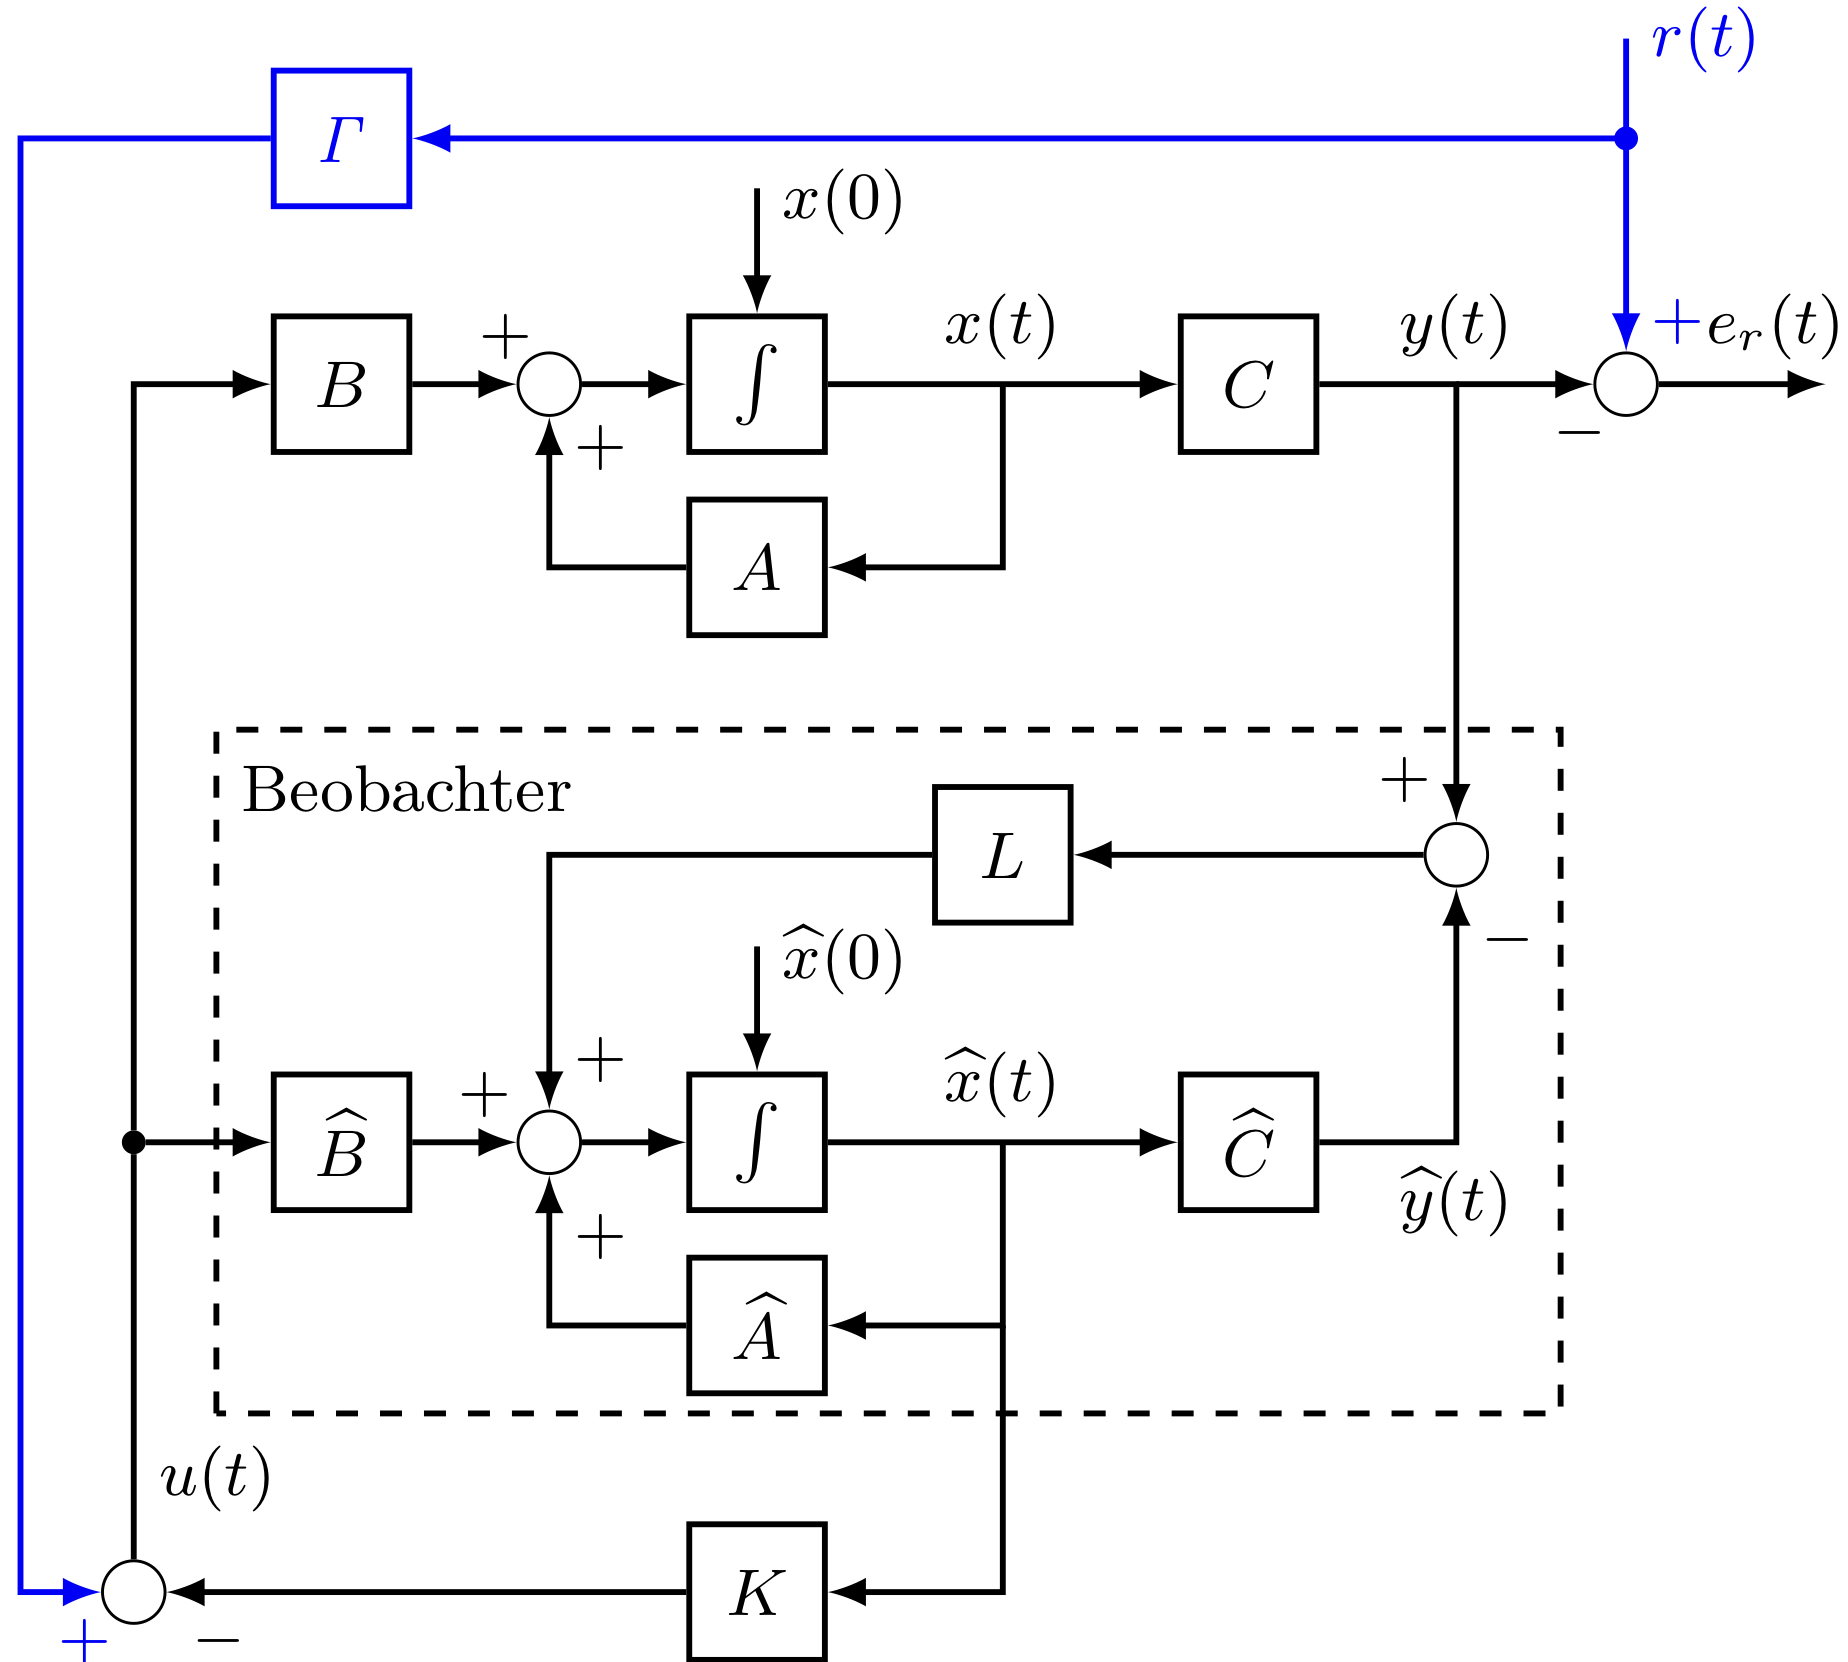
\includegraphics[width = 0.6\linewidth]{images/10/LQG_Folg_Vorst.jpeg}
            \caption{LQG Folgeregelung durh Vorsteuerung}
        \end{figure}
        Daraus ergeben sich folgende steady-state Gleichungen
        \begin{align*}
            0 &= A\cdot x_\infty + B\cdot u_\infty\\
            r(t) &= C\cdot x_\infty\\
            \Rightarrow \begin{bmatrix}0\\r(t)\end{bmatrix} &= 
            \underbrace{\begin{bmatrix}
            A & B\\
            C & 0
            \end{bmatrix}}_{F} \cdot
            \begin{bmatrix}x_\infty\\u_\infty\end{bmatrix}
        \end{align*}
        Falls $F$ vollen rang hat, kann man für $r(t)\rightarrow\{x_\infty,\, u_\infty\}$ folgende Beziehung herleiten.
        \begin{align*}
            u_\infty + K\cdot x_\infty &= \underbrace{-\Big(C\cdot\big(A-B\cdot K\big)^{-1}\cdot B\Big)^{-1}}_{\mathit{\Gamma}} \cdot r(t)\\
            &= \mathit{\Gamma}\cdot r(t)
        \end{align*}